\chapter{Testovanie}

V tejto kapitole zhrnieme ako bola aplikácia testovaná a aké výsledky vyplynuli z testovania. 

\begin{figure}[!b]
\centerline{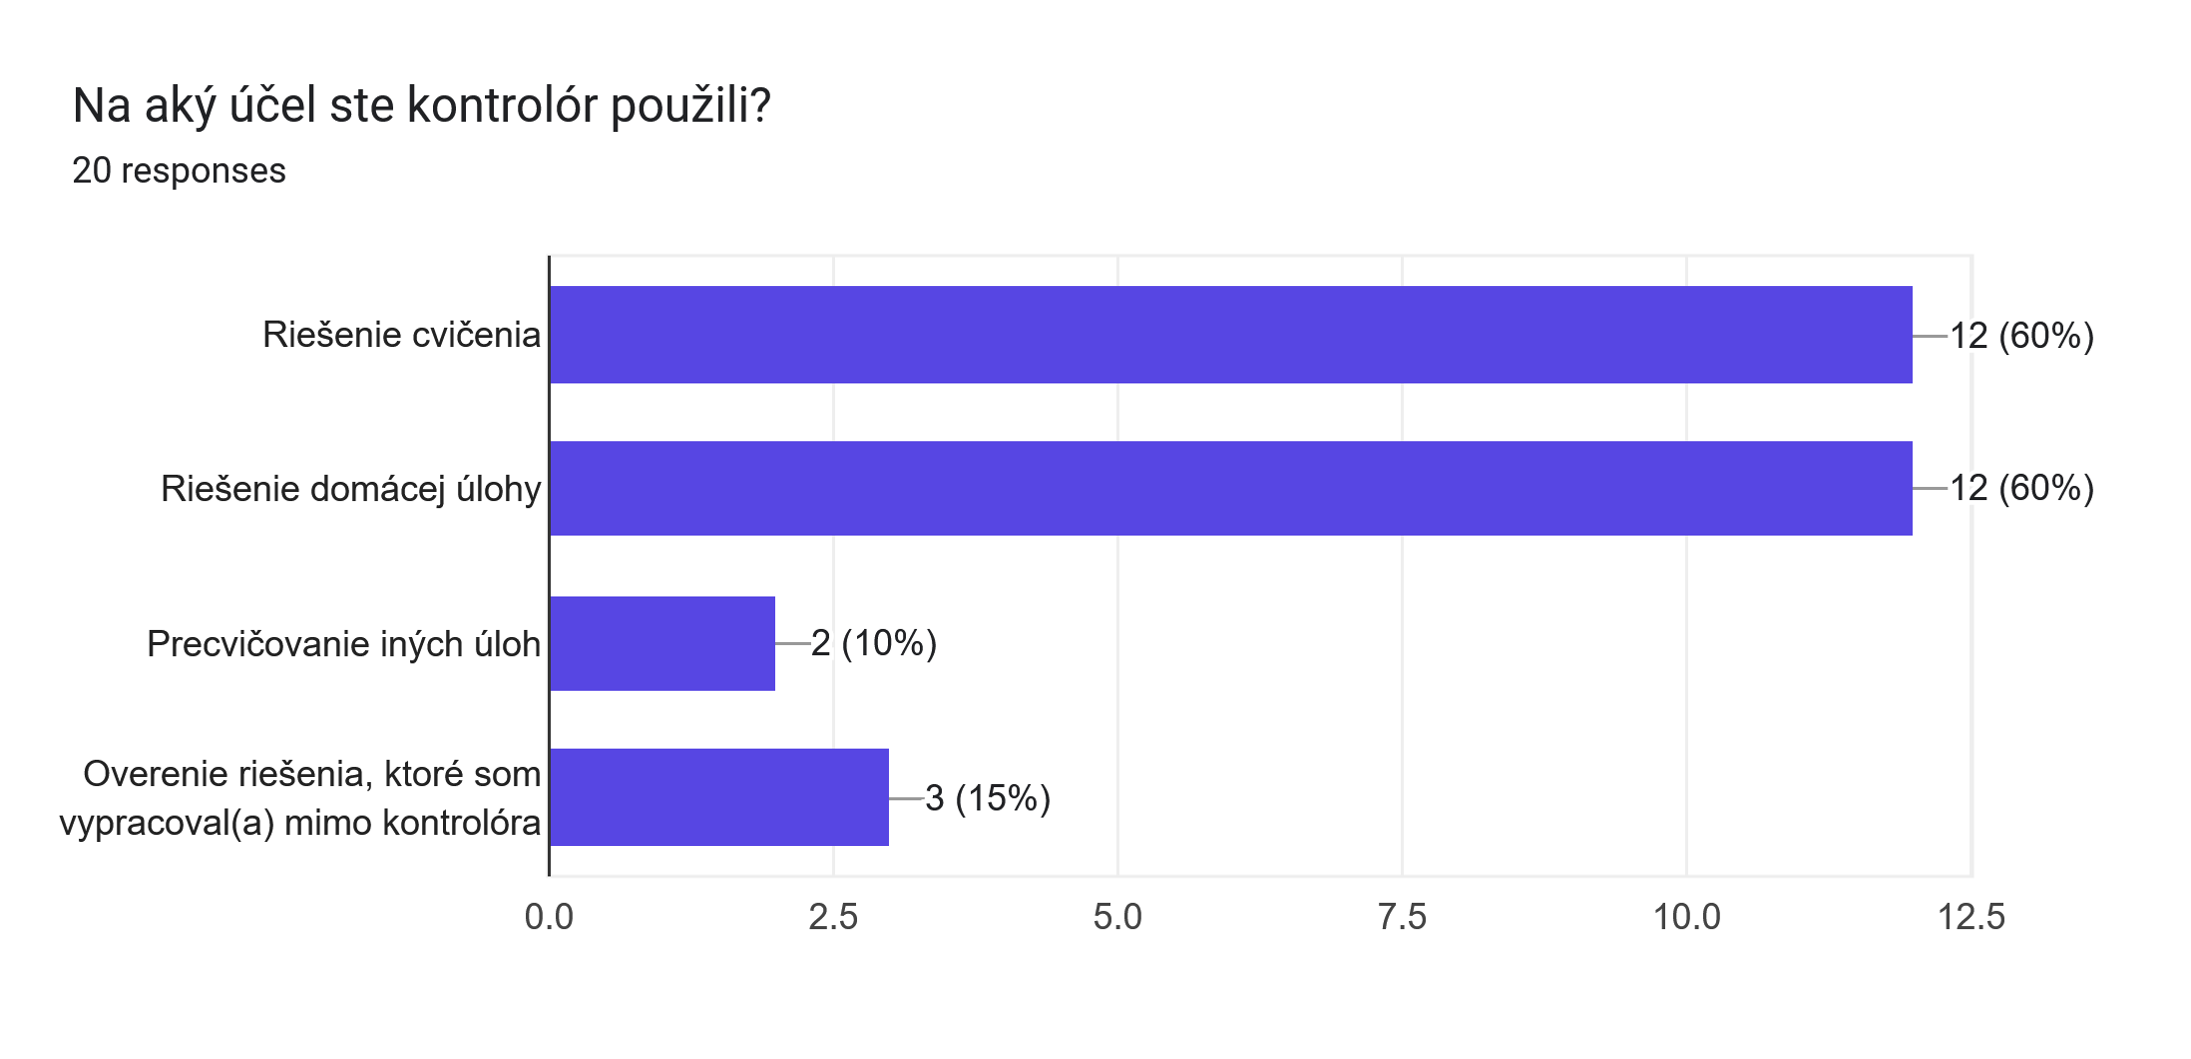
\includegraphics[width=\textwidth]{images/formResponse1}}
\caption[Graf odpovedí na otázku Na aký účel ste kontrolór použili?]{Na aký účel ste kontrolór použili? Výsledky sú v počte študentov}
\label{obr:FormResponse1}
\end{figure}

\section{Spôsob testovania}

Aplikácia bola testovaná počas letného semestra v rámci predmetu Logika pre informatikov ako súčasť cvičení a domácej úlohy. Súčasťou domácej úlohy pre študentov bola úloha na úpravu formúl do prvorádovej CNF. Zadanie úlohy je v prílohe A \eqref{appendA}. Keďže aplikácia nebola v ten čas integrovaná do elektronického pracovného zošita, aplikácia bola študentom zverejnená cez stránku GitHub. Nasledovné študenti mali možnosť vyplniť dotazník o ich skúsenostiach s aplikáciou. Kópia dotazníka sa nachádza v prílohe B \eqref{appendB}.

\newpage 

Dotazník sa skladal z pätnástich otázok, z ktorých prvé tri sa zaoberali spôsobom, akým študenti použili aplikáciu. Potom nasledovalo desať otázok podľa štandardu SUS \cite{SUS}. Dotazník štandardu SUS obsahuje desať otázok na ktoré, je možné odpovedať piatimi odpoveďami od \uv{úplne nesúhlasím} po \uv{úplne súhlasím}. Každá odpoveď je ohodnotená číslom 1 až 5, kde úplne súhlasím je za 5 bodov. Z odpovedí sa vypočíta SUS skóre, ktoré zodpovedá používateľnosti aplikácie. Čím vyššie je SUS skóre, tým je aplikácia používateľnejšia. Posledné dve otázky boli otvorené, študenti v nich mohli vyjadriť konkrétne čo sa im páčilo, respektíve nepáčilo na aplikácii.


\section{Výsledky testovania}


\begin{figure}[!b]
\centerline{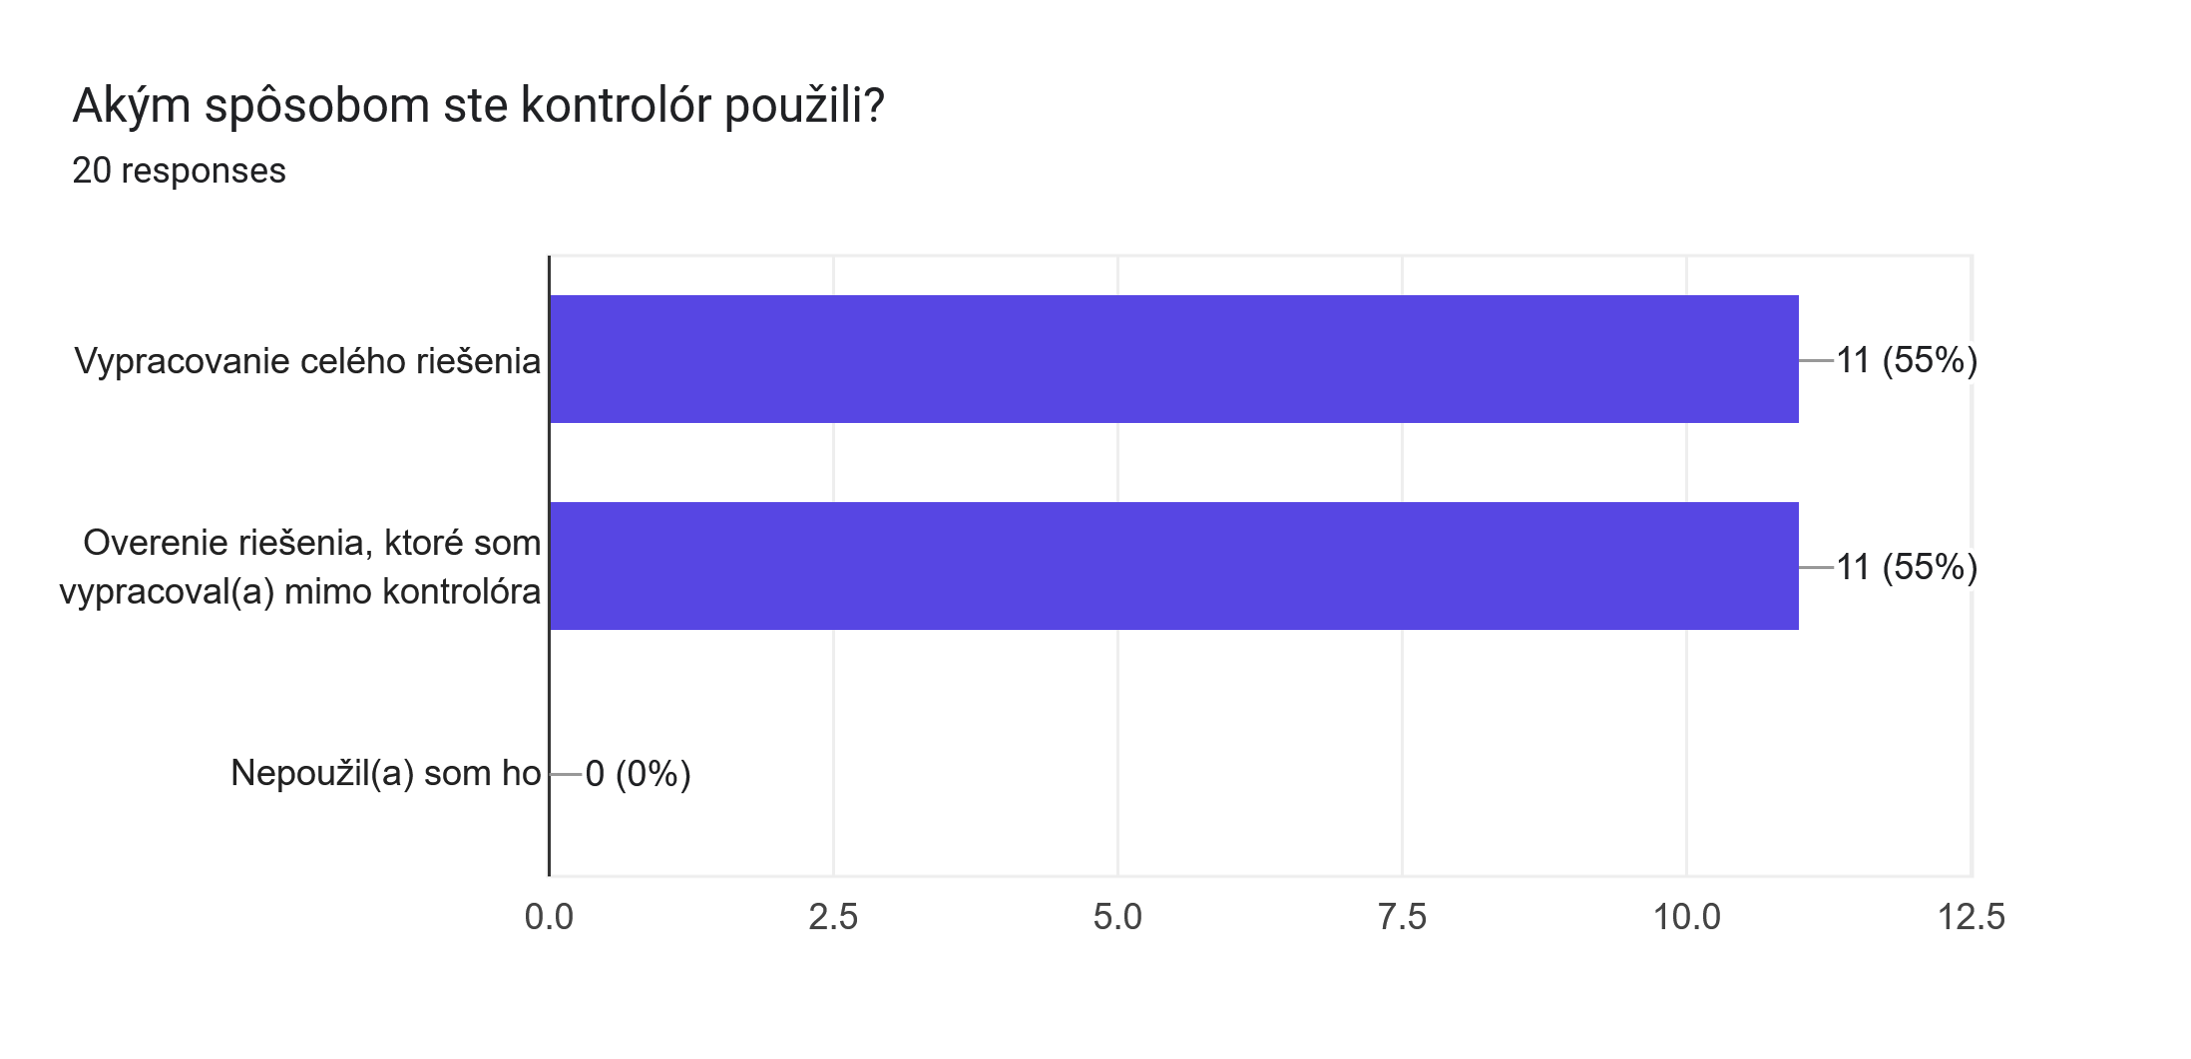
\includegraphics[width=\textwidth]{images/formResponse2}}
\caption[Graf odpovedí na otázku Akým spôsobom ste kontrolór použili?]{Akým spôsobom ste kontrolór použili? Výsledky sú v počte študentov}
\label{obr:FormResponse2}
\end{figure}

Dotazník vyplnilo 20 študentov, pričom všetci aplikáciu použili. Na grafe v obrázku \ref{obr:FormResponse1} vidno, že najčastejšie použitie aplikácie, bolo pre riešenie zadaných úloh. Pár študentov tiež použili aplikáciu pre precvičovanie iných úloh. Graf na obrázku \ref{obr:FormResponse2} ukazuje, že iba približne polovica študentov použila aplikáciu pre vypracovanie celého riešenia. Veľká časť respondentov ju použila pre overenie ich riešenia. Je pravdepodobné, že ak by bola aplikácia počas testovania integrovaná do Logic Workbooku, tak by časť študentov, ktorý aplikáciu požili pre celé riešenie vzrástla.

Pri počítaní SUS skóre, každá nepárna otázka je sformulovaná pozitívne a prispieva svojou hodnotou k skóre. Naopak každá párna otázka je sformulovaná negatívne a znižuje skóre. Vypočítané priemerné SUS skóre vyšlo 72.875 čo znamená, že použiteľnosť aplikácie je dobrá. Najlepšie skóre mala otázka \uv{Vedel(a) som si predstaviť, že väčšina ľudí sa naučí používať kontrolór veľmi rýchlo.}. Otázka mala priemernú hodnotu 4.15 čo znamená, že v priemere študenti súhlasili s touto otázkou. V otvorenej časti formulára viacerý študenti napísali, že sa im na aplikácii páčila jej jednoduchosť. Pár študentov ocenili, že aplikácia kontroluje samostatné ekvivalentné úpravy, a že používať aplikáciu bolo lepšie ako meniť formuly ručne.

Najhoršie skóre mala otázka \uv{Potreboval(a) som sa naučiť mnoho vecí predtým, ako som mohol(a) začať pracovať s kontrolórom.}. Otázka mala priemernú hodnotou 2.2, čiže študenti v priemere nesúhlasili s tvrdením. Najčastejšou pripomienkou bolo to, že chybové hlášky neboli dosť nápomocné. Táto pripomienka sa dá riešiť iba do určitej miery, lebo s konkrétnejšími chybovými hláškami rastie šanca, že aplikácia zle určí kde vznikla chyba, čo môže študentov zmiasť. 








